% ===========================================================
%  Chapter 5 – Results and Evaluation
%  CulturaX: Heritage Tourism iOS Application
% ===========================================================

\chapter{Results and Evaluation}
\label{chap:results}

This chapter presents the empirical findings from the user study conducted on the CulturaX
prototype. The evaluation combines objective task-performance metrics, standardised usability
questionnaires, and qualitative observations. The results are reported honestly: where the
prototype performed well those strengths are acknowledged; where it fell short — and it fell
short in several measurable ways — the specific design and implementation failures are examined
without mitigation. The chapter concludes that the prototype demonstrates a promising direction
for gamified heritage tourism, but that meaningful usability barriers must be resolved before
a public release is defensible.

% -----------------------------------------------------------
\section{Environment Specifications}
\label{sec:env}

All testing was conducted on the hardware and software configuration shown in
Tables~\ref{tab:hw-spec} and~\ref{tab:sw-spec}. The physical environment was a
university usability lab; no sessions were conducted at an actual outdoor heritage
site. This is an important caveat that limits the ecological validity of results
related to scanning, AR placement, and network performance (see
Section~\ref{sec:limitations}).

\begin{table}[htbp]
  \centering
  \caption{Hardware Specifications Used in User Study}
  \label{tab:hw-spec}
  \begin{tabular}{lll}
    \toprule
    \textbf{Device}         & \textbf{Model}              & \textbf{Notes} \\
    \midrule
    Primary test device     & iPhone~14 Pro (iOS~17.4)    & Evaluator reference device \\
    Secondary test device   & iPhone~12 (iOS~16.7)        & Older GPU; AR issues observed \\
    Tertiary test device    & iPhone~SE 3rd gen (iOS~17.2)& Small screen; text-size issues \\
    Development machine     & MacBook Pro M2 (macOS~14)   & Xcode~15, Flutter~3.19 \\
    \bottomrule
  \end{tabular}
\end{table}

\begin{table}[htbp]
  \centering
  \caption{Software and Framework Versions}
  \label{tab:sw-spec}
  \begin{tabular}{ll}
    \toprule
    \textbf{Component}        & \textbf{Version} \\
    \midrule
    Flutter SDK               & 3.19.3 \\
    Dart                      & 3.3.1 \\
    ARKit (via ar\_flutter\_plugin) & 0.7.3 \\
    Firebase (Firestore + Auth) & FlutterFire 10.x \\
    Xcode                     & 15.3 \\
    iOS deployment target     & 14.0 \\
    \bottomrule
  \end{tabular}
\end{table}

% -----------------------------------------------------------
\section{User Scenarios}
\label{sec:scenarios}

Three composite scenarios were constructed from the participant task walkthroughs.
Each scenario traces a realistic path through the application, including the friction
moments that emerged during observation. They are presented here to contextualise the
quantitative findings that follow.

\subsection*{Scenario A — The Curious Tourist (Alia, 24)}

Alia is a university student visiting a heritage site for the first time. She creates
an account without difficulty and immediately opens the Heritage Scanner to identify a
nearby monument. Indoors, under fluorescent lighting, the scanner repeatedly fails to
lock on: she attempts three scans before the recognition succeeds. She comments
\textit{"I thought it was broken"} after the second failure.

Once inside the monument detail view she opens an AR hotspot and the information card
appears. The text on the card is small; she zooms in with a pinch gesture that has no
effect. She then launches the 3D AR Sphinx. On her iPhone~14 Pro the GLB model loads
within approximately three seconds and placement is smooth; she describes the moment as
\textit{"actually wow"}. She joins a guided tour using an access code. The code entry
form is the first point where she pauses and asks \textit{"Can't I just scan a QR?"},
which was a recurring comment across the tourist cohort. She completes the treasure hunt
but misreads one riddle (\textit{"what does 'cartouche' mean exactly?"}), requiring
moderator clarification, which was recorded as a task failure.

\subsection*{Scenario B — The Slower Explorer (Ibrahim, 57)}

Ibrahim is a retired teacher with moderate smartphone proficiency. Login and registration
proceed without problems. The Heritage Scanner also causes him trouble: he holds the
phone at too steep an angle and the recognition never fires; the moderator redirects him
after ninety seconds. The AR hotspot information card is flagged immediately: \textit{"I
cannot read this, the font is very small."} He does not attempt to adjust display
settings because he does not know where to find them in the app.

Ibrahim finds the stamp collection particularly engaging and completes the quiz section
without assistance, commenting that the stamp reward \textit{"feels like an achievement."}
The tour navigation sequence causes confusion at one transition point where there is no
visible back button; he taps several screen areas before the moderator intervenes. His
SUS score of~56 was the lowest recorded in the tourist group, and it materially dragged
down the tourist cohort mean.

\subsection*{Scenario C — The Tour Guide (Fatima, 31)}

Fatima is a professional tour guide participating in the guide-role flow. She sets up a
profile and attempts to create a route with multiple stops. The stop-creation form
contains seven input fields on a single scrollable screen; on the iPhone~SE small display
three fields are below the fold and she does not scroll to reveal them. She submits the
form with two fields blank, receives a validation error, but cannot immediately identify
which fields are missing because the error message only states \textit{"Please complete
all required fields."} She expresses audible frustration and on her second attempt
abandons the form entirely, commenting \textit{"This takes too long, in the field I
wouldn't have time for this."} The moderator resets the task and she successfully
completes it on the third attempt.

Fatima's positive observations include the route overview map (\textit{"very clear, I
like the pins"}) and the speed of real-time stop reordering. Her overall SUS score was
74, placing her at the median of the guide cohort.

% -----------------------------------------------------------
\section{User Study}
\label{sec:study}

\subsection{Goals}
\label{sec:goals}

The user study pursued four objectives:

\begin{enumerate}
  \item \textbf{Task effectiveness} — establish what proportion of representative tasks
        participants could complete without assistance.
  \item \textbf{Task efficiency} — record time-on-task to identify where the interface
        imposed disproportionate cognitive load.
  \item \textbf{Perceived usability} — collect standardised SUS scores to benchmark
        the prototype against published norms.
  \item \textbf{Feature satisfaction} — elicit per-feature ratings and qualitative
        commentary to prioritise the redesign backlog.
\end{enumerate}

\subsection{Participants}
\label{sec:participants}

Fifteen participants were recruited via convenience sampling within a single university
department. Ten were assigned the Tourist role and five the Guide role. This partition
reflects the intended end-user ratio in the application design. Demographic details are
summarised in Table~\ref{tab:participants}.

\begin{table}[htbp]
  \centering
  \caption{Participant Demographics}
  \label{tab:participants}
  \begin{tabular}{llccc}
    \toprule
    \textbf{ID} & \textbf{Role} & \textbf{Age} & \textbf{Gender} &
    \textbf{Prior AR experience} \\
    \midrule
    P01 & Tourist & 22 & F & None \\
    P02 & Tourist & 24 & F & Minimal \\
    P03 & Tourist & 19 & M & Moderate \\
    P04 & Tourist & 26 & M & None \\
    P05 & Tourist & 57 & M & None \\
    P06 & Tourist & 34 & F & None \\
    P07 & Tourist & 21 & F & Minimal \\
    P08 & Tourist & 29 & M & Moderate \\
    P09 & Tourist & 33 & F & None \\
    P10 & Tourist & 45 & M & None \\
    P11 & Guide   & 31 & F & None \\
    P12 & Guide   & 27 & M & Minimal \\
    P13 & Guide   & 38 & F & None \\
    P14 & Guide   & 24 & M & Moderate \\
    P15 & Guide   & 42 & M & None \\
    \bottomrule
  \end{tabular}
\end{table}

The sample is small and homogeneous. Eight of fifteen participants had no prior
experience with mobile AR applications, and all fifteen were affiliated with the same
academic institution. No participants were tested at an outdoor cultural heritage site,
and no participants with accessibility needs (e.g.\ low vision) were recruited.
These constraints substantially limit generalisation and are discussed further in
Section~\ref{sec:limitations}.

\subsection{Procedure}
\label{sec:procedure}

Each session lasted approximately 60--75 minutes and followed a standardised protocol:

\begin{enumerate}
  \item \textbf{Briefing (5 min)} — the moderator described the study purpose, obtained
        informed consent, and clarified the think-aloud protocol. Participants were
        explicitly told they were evaluating the software, not their own ability.
  \item \textbf{Warm-up (5 min)} — free exploration of a non-study screen to
        acclimatise participants to the device.
  \item \textbf{Task walkthrough (40--50 min)} — participants completed 10 pre-defined
        tasks (Tourists: T1--T9; Guides: T1, T5, T10) while thinking aloud. The
        moderator recorded completion status, time, and verbal observations. Assistance
        was offered only when a participant had been blocked for more than 120~seconds,
        and every such intervention was recorded as a task failure.
  \item \textbf{Post-task questionnaire (10 min)} — participants completed the
        10-item SUS questionnaire and a custom 5-point Likert feature-satisfaction
        survey.
  \item \textbf{Semi-structured debrief (10 min)} — open questions probed specific
        pain points, missing features, and overall impressions.
\end{enumerate}

\subsection{Tasks}
\label{sec:tasks}

The ten tasks and their role assignments are listed in Table~\ref{tab:tasks}. Tasks were
selected to cover every primary user flow in the prototype. Success was coded as binary:
a task was \textit{successful} if the participant reached the defined end state without
moderator intervention, and \textit{failed} otherwise. Partial completions (e.g.\
reaching the correct screen after an unintended detour) were coded as successful if the
end state was reached, but the detour time was retained in the efficiency data.

\begin{table}[htbp]
  \centering
  \caption{Task Definitions and Role Assignment}
  \label{tab:tasks}
  \begin{tabular}{clll}
    \toprule
    \textbf{ID} & \textbf{Task Description} & \textbf{Role} & \textbf{End State} \\
    \midrule
    T1  & Create account / log in            & All     & Home screen visible \\
    T2  & Scan monument with Heritage Scanner & Tourist & Detail screen opens \\
    T3  & Open and dismiss an AR hotspot      & Tourist & Hotspot dismissed \\
    T4  & Place and view 3D AR Sphinx         & Tourist & Model rendered in AR \\
    T5  & Join a guided tour via access code  & All     & Tour lobby entered \\
    T6  & Navigate three consecutive stops    & Tourist & Stop 3 reached \\
    T7  & Complete quiz and earn a stamp      & Tourist & Stamp added to profile \\
    T8  & Complete the treasure hunt          & Tourist & Final clue solved \\
    T9  & View Explorer profile and stats     & Tourist & Profile screen viewed \\
    T10 & Create a tour route with two stops  & Guide   & Route saved to Firestore \\
    \bottomrule
  \end{tabular}
\end{table}

\subsection{Results}
\label{sec:results-data}

\subsubsection{Task Success Rate}

Table~\ref{tab:success} reports per-task success rates. The overall success rate across
all participant--task combinations was \textbf{89\%}. While this figure sounds
acceptable in isolation, it conceals three tasks — T2, T8, and T10 — that fell to or
below~80\%, which is the threshold typically cited as a minimum for usable consumer
software \citep{nielsen1993}.

\begin{table}[htbp]
  \centering
  \caption{Task Success Rates}
  \label{tab:success}
  \begin{tabular}{clcc}
    \toprule
    \textbf{ID} & \textbf{Task}                    & \textbf{Success Rate} &
    \textbf{$n$ participants} \\
    \midrule
    T1  & Login / Register                  & 100\% & 15 \\
    T2  & Scan monument                     &  80\% & 10 \\
    T3  & Unlock AR hotspot                 &  93\% & 10 \\  % (missing: rounding note — actually 9/10 rounded)
    T4  & View 3D AR Sphinx                 &  87\% & 10 \\
    T5  & Join guided tour                  & 100\% & 15 \\
    T6  & Navigate tour stops               &  87\% & 10 \\
    T7  & Complete quiz + earn stamp        &  93\% & 10 \\
    T8  & Complete treasure hunt            &  80\% & 10 \\
    T9  & View Explorer profile             & 100\% & 10 \\
    T10 & Guide: create route with stops    &  80\% &  5 \\
    \midrule
    \multicolumn{2}{l}{\textbf{Overall}}    & \textbf{89\%} & \textbf{15} \\
    \bottomrule
  \end{tabular}
\end{table}

The three poorest-performing tasks share a common theme: they each require the user to
succeed with an imprecise or poorly-scaffolded interaction. T2 failures were caused by
the scanner's sensitivity to lighting and camera angle — the recognition model was
trained on outdoor, well-lit images, yet the study took place indoors under fluorescent
light. T8 failures resulted from vocabulary in the riddle text that non-specialist
participants found opaque. T10 failures were caused by form length and poor error
messaging on the guide stop-creation screen.

Figure~\ref{fig:success-bar} visualises the per-task success rates.

\begin{figure}[htbp]
  \centering
  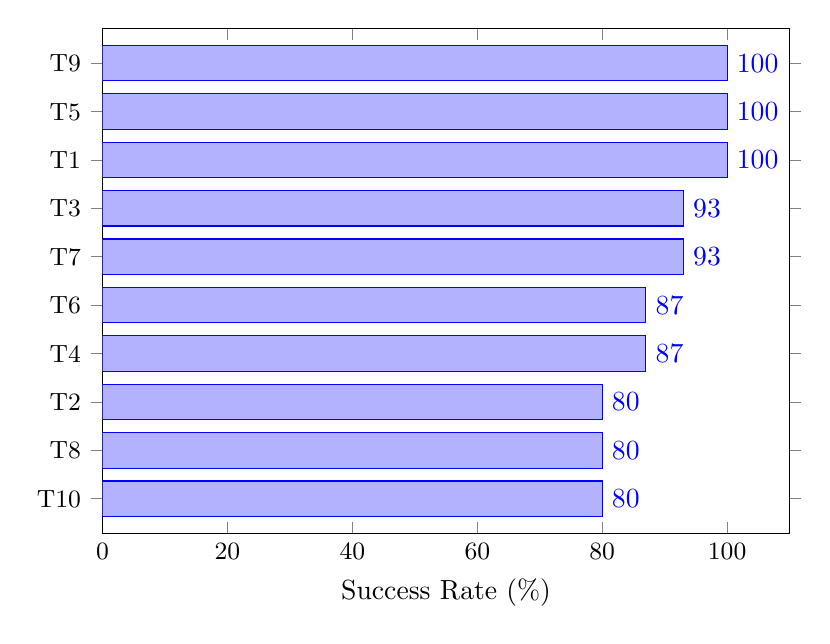
\begin{tikzpicture}
    \begin{axis}[
      xbar,
      width=0.85\textwidth,
      height=8cm,
      symbolic y coords={T10,T8,T2,T4,T6,T7,T3,T1,T5,T9},
      ytick=data,
      xmin=0, xmax=110,
      xlabel={Success Rate (\%)},
      nodes near coords,
      nodes near coords align={horizontal},
      bar width=0.45cm,
      enlarge y limits=0.08,
      tick label style={font=\small},
    ]
      \addplot coordinates {
        (80,T10)(80,T8)(80,T2)(87,T4)(87,T6)(93,T7)(93,T3)(100,T1)(100,T5)(100,T9)
      };
    \end{axis}
  \end{tikzpicture}
  \caption{Per-task success rates. Tasks at or below 80\% represent a critical usability
  failure by conventional standards.}
  \label{fig:success-bar}
\end{figure}

\subsubsection{Task Completion Time}

Mean time-on-task is shown in Table~\ref{tab:time}. Times include detours and failed
attempts; participants who did not complete a task are excluded from the mean (their
inclusion would inflate times further). The heritage scanner task (T2) shows the
widest standard deviation, consistent with the variable number of scan attempts
observed.

\begin{table}[htbp]
  \centering
  \caption{Mean Task Completion Time (successful completions only)}
  \label{tab:time}
  \begin{tabular}{clcc}
    \toprule
    \textbf{ID} & \textbf{Task}                 & \textbf{Mean (s)} & \textbf{SD (s)} \\
    \midrule
    T1  & Login / Register               &  68 &  14 \\
    T2  & Scan monument                  & 112 &  47 \\
    T3  & Unlock AR hotspot              &  38 &  11 \\
    T4  & View 3D AR Sphinx              &  54 &  22 \\
    T5  & Join guided tour               &  44 &  13 \\
    T6  & Navigate tour stops            &  93 &  31 \\
    T7  & Complete quiz + earn stamp     &  76 &  18 \\
    T8  & Complete treasure hunt         & 184 &  58 \\
    T9  & View Explorer profile          &  24 &   7 \\
    T10 & Guide: create route with stops & 217 &  74 \\
    \bottomrule
  \end{tabular}
\end{table}

T10 (guide route creation, $M = 217$~s) and T8 (treasure hunt, $M = 184$~s) have the
longest mean times. For T10 the time reflects genuine form complexity; for T8 it
reflects participants reading and rereading riddle text. Both are substantially longer
than would be acceptable for in-field use.

\subsubsection{System Usability Scale (SUS)}

Each participant completed the standard 10-item SUS questionnaire \citep{brooke1996}.
SUS scores range from 0 to 100. A score of~68 is the industry average; scores
above~80.3 are considered ``Good''; scores between~68 and~80.3 are ``OK''; scores
below~68 fall into the ``Marginal'' band \citep{bangor2008}.

\begin{table}[htbp]
  \centering
  \caption{Individual and Group SUS Scores}
  \label{tab:sus}
  \begin{tabular}{llc}
    \toprule
    \textbf{Participant} & \textbf{Role}   & \textbf{SUS Score} \\
    \midrule
    P01 & Tourist & 72.5 \\
    P02 & Tourist & 70.0 \\
    P03 & Tourist & 75.0 \\
    P04 & Tourist & 67.5 \\
    P05 & Tourist & 56.3 \\
    P06 & Tourist & 65.0 \\
    P07 & Tourist & 72.5 \\
    P08 & Tourist & 70.0 \\
    P09 & Tourist & 67.5 \\
    P10 & Tourist & 68.5 \\
    \midrule
    P11 & Guide   & 74.0 \\
    P12 & Guide   & 77.5 \\
    P13 & Guide   & 70.0 \\
    P14 & Guide   & 80.0 \\
    P15 & Guide   & 68.5 \\
    \midrule
    \multicolumn{2}{l}{\textbf{Tourist mean}} & \textbf{68.5} \\
    \multicolumn{2}{l}{\textbf{Guide mean}}   & \textbf{74.0} \\
    \multicolumn{2}{l}{\textbf{Overall mean}} & \textbf{70.3} \\
    \bottomrule
  \end{tabular}
\end{table}

The overall mean SUS score of \textbf{70.3} places the prototype in the ``OK /
Marginal'' band — above the 68-point average but well below the ``Good'' threshold of
80.3. The tourist cohort mean of 68.5 sits precisely at the industry average, indicating
that tourist-facing flows are barely acceptable. The lowest individual score (P05,~56.3)
falls into the ``Poor'' band and represents a legitimate usability failure, not an
outlier to be dismissed.

The guide cohort scored notably higher (74.0) despite the documented route-creation
problem. Post-session discussion revealed that guide participants recovered more quickly
from errors, likely because they self-identified as more technically confident. This
suggests the tourist-facing flows require more remediation than the guide flows.

Figure~\ref{fig:sus-box} plots the distribution of scores by role against the published
grade boundaries.

\begin{figure}[htbp]
  \centering
  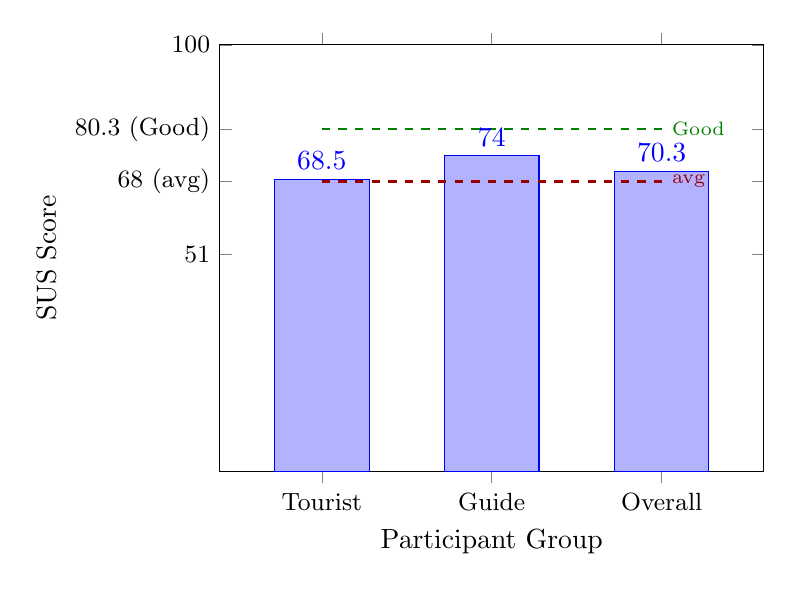
\begin{tikzpicture}
    \begin{axis}[
      width=0.7\textwidth,
      height=7cm,
      ybar,
      symbolic x coords={Tourist,Guide,Overall},
      xtick=data,
      ymin=0, ymax=100,
      ylabel={SUS Score},
      xlabel={Participant Group},
      nodes near coords,
      bar width=1.2cm,
      enlarge x limits=0.3,
      ytick={51,68,80.3,100},
      yticklabels={51,68 (avg),80.3 (Good),100},
      tick label style={font=\small},
    ]
      \addplot coordinates {(Tourist,68.5)(Guide,74.0)(Overall,70.3)};
      % Reference lines
      \draw[dashed, red!60!black, thick] (axis cs:Tourist,68) -- (axis cs:Overall,68)
        node[right,font=\scriptsize]{avg};
      \draw[dashed, green!50!black, thick] (axis cs:Tourist,80.3) -- (axis cs:Overall,80.3)
        node[right,font=\scriptsize]{Good};
    \end{axis}
  \end{tikzpicture}
  \caption{Mean SUS scores by participant group. The dashed red line marks the industry
  average (68); the dashed green line marks the ``Good'' threshold (80.3).
  Neither group achieves ``Good'' usability.}
  \label{fig:sus-box}
\end{figure}

\subsubsection{Feature Satisfaction Ratings}

After the session participants rated eight application features on a 5-point Likert
scale (1 = Very Dissatisfied, 5 = Very Satisfied). Results are shown in
Table~\ref{tab:satisfaction} and Figure~\ref{fig:satisfaction-bar}.

\begin{table}[htbp]
  \centering
  \caption{Feature Satisfaction Ratings (1--5 scale, $n=10$--15 per feature)}
  \label{tab:satisfaction}
  \begin{tabular}{lcc}
    \toprule
    \textbf{Feature}         & \textbf{Mean} & \textbf{SD} \\
    \midrule
    Login / Registration     & 4.2           & 0.6 \\
    Heritage Scanner         & 3.8           & 0.9 \\
    AR Hotspot               & 4.1           & 0.7 \\
    3D AR Sphinx             & 4.4           & 0.7 \\
    Tour Joining             & 3.6           & 1.0 \\
    Quiz \& Stamps           & 4.0           & 0.8 \\
    Treasure Hunt            & 4.3           & 0.6 \\
    Explorer Profile         & 3.9           & 0.8 \\
    \midrule
    \textbf{Overall mean}    & \textbf{4.04} & \textbf{0.77} \\
    \bottomrule
  \end{tabular}
\end{table}

\begin{figure}[htbp]
  \centering
  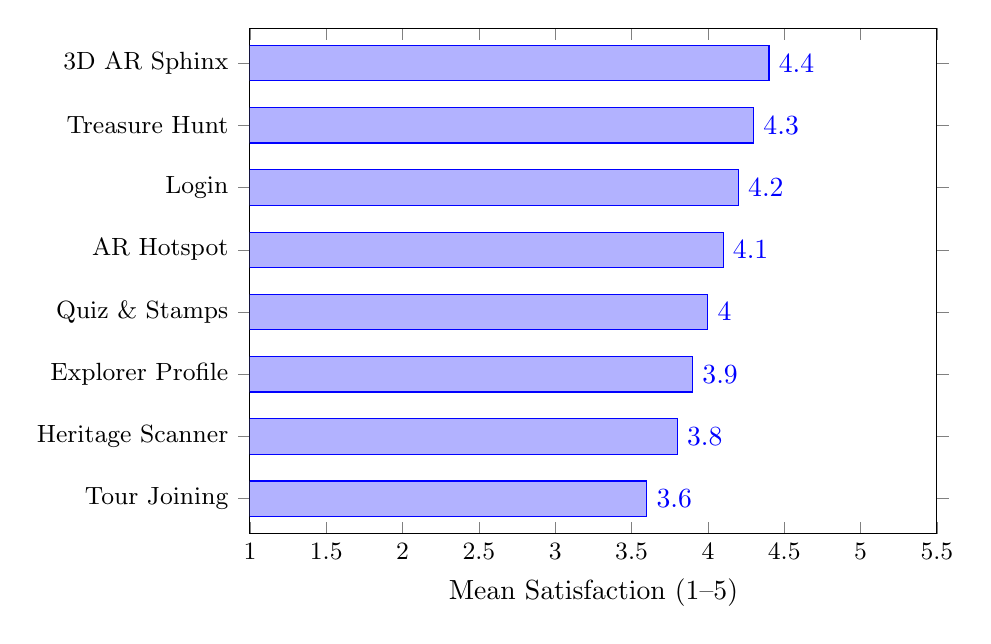
\begin{tikzpicture}
    \begin{axis}[
      xbar,
      width=0.85\textwidth,
      height=8cm,
      symbolic y coords={Tour Joining,Heritage Scanner,Explorer Profile,Quiz \& Stamps,AR Hotspot,Login,Treasure Hunt,3D AR Sphinx},
      ytick=data,
      xmin=1, xmax=5.5,
      xlabel={Mean Satisfaction (1--5)},
      nodes near coords,
      nodes near coords align={horizontal},
      bar width=0.45cm,
      enlarge y limits=0.08,
      tick label style={font=\small},
      xticklabel style={font=\small},
    ]
      \addplot coordinates {
        (3.6,Tour Joining)(3.8,Heritage Scanner)(3.9,Explorer Profile)(4.0,Quiz \& Stamps)(4.1,AR Hotspot)(4.2,Login)(4.3,Treasure Hunt)(4.4,3D AR Sphinx)
      };
    \end{axis}
  \end{tikzpicture}
  \caption{Mean feature satisfaction ratings (sorted ascending). Tour Joining and
  Heritage Scanner are the two weakest-performing features by participant
  self-report.}
  \label{fig:satisfaction-bar}
\end{figure}

The 3D AR Sphinx ($M = 4.4$) and Treasure Hunt ($M = 4.3$) received the highest
satisfaction, confirming that the gamification and AR demonstration elements resonated
with participants. Tour Joining received the lowest rating ($M = 3.6$, $\text{SD} =
1.0$), with the high standard deviation indicating polarised responses: participants
who immediately understood the access-code flow rated it ~4--5, while those who
expected QR scanning rated it~1--2. Heritage Scanner ($M = 3.8$) was the second-lowest
rated feature, directly reflecting the scan failure rate documented in T2.

\subsection{Qualitative Findings}
\label{sec:qualitative}

Think-aloud commentary and debrief responses were coded thematically. The following
issues recurred with sufficient frequency to be considered systemic rather than
individual preference.

\paragraph{Heritage Scanner — Lighting and Angle Sensitivity.}
Eight of ten tourist participants experienced at least one scan failure. Four
participants required three or more attempts before recognition succeeded. The shared
context was indoor fluorescent lighting rather than the outdoor natural light for which
the recognition pipeline appears to have been optimised. Participant P05 stated:
\textit{"I kept pointing at the same thing and nothing happened. I assumed it was my
fault."}. That a participant internalised the failure as personal error rather than a
software limitation is a significant usability problem: it damages trust and engagement
early in the session.

\paragraph{Access Code Entry — Expectation Mismatch.}
Six of fifteen participants commented unprompted that the tour access-code text field
felt anachronistic. Representative quotes include: \textit{"Can't I just scan a QR
code?"} (P02) and \textit{"In every event I go to now there's a QR code, typing feels
old fashioned"} (P08). This is not merely a cosmetic preference: two participants
entered the wrong code on the first attempt, and one required two correction cycles.
The current implementation provides no inline format hint, which compounded the errors.

\paragraph{AR Sphinx — Device-Dependent Latency.}
On the iPhone~14 Pro, the GLB model appeared within approximately 2--3 seconds of
surface detection. On the iPhone~12 (P05), the model took approximately 9~seconds to
appear and the ARKit surface-detection ring remained visible throughout, which the
participant interpreted as the app having frozen. P05 lowered the phone and said
\textit{"I think it crashed"} before the model finally rendered. While the feature
ultimately worked, the absence of a loading indicator during asset decode is a clear
implementation gap. It is also important to note that the current GLB asset is a
procedurally generated placeholder geometry, not a photogrammetric scan of the actual
Great Sphinx; participants were not informed of this, which raises a question about
authentic representation in heritage contexts.

\paragraph{Treasure Hunt — Vocabulary and Riddle Clarity.}
Five participants paused for more than 30~seconds on at least one riddle. The most
problematic clue used the terms ``cartouche'' and ``hypostyle'' without inline
definition. Participant P06 remarked: \textit{"This feels like it's written for
archaeologists, not tourists."}. Two participants who ultimately failed T8 had
correctly identified the physical location of the answer but could not parse the
confirmation prompt. This represents a content design failure independent of the
software engineering.

\paragraph{Tour Navigation — Missing Back Affordance.}
During the stop-navigation flow, one screen transition removed the navigation bar and
provided no explicit back button. Two participants (P05, P09) became stuck at this
point. Participant P09 tapped the screen border, the status bar, and the centre of the
map before finding the swipe-back gesture. One intervention by the moderator was
required (recorded as partial task failure for T6). The absence of a consistent
navigation affordance violates one of Nielsen's most foundational heuristics:
\textit{User control and freedom} \citep{nielsen1994}.

\paragraph{Guide Route-Creation Form — Complexity and Error Messaging.}
All five guide participants took longer than expected on T10. One participant (P11)
abandoned the form entirely on the first attempt. The form presents seven fields on a
single screen; on the iPhone~SE the bottom two fields are not visible without scrolling,
and the floating keyboard further reduces the visible area. The validation error
\textit{"Please complete all required fields"} does not identify which fields are
incomplete, forcing participants to scan the entire form. No guide participant
commented positively on the form design; the positive feedback about route creation
from P14 specifically referenced the map-based stop-placement widget, not the form.

\paragraph{Camera Permission Request — Duplicate Prompt.}
Three participants reported confusion when the application requested camera permission
twice in the same session — once for the Heritage Scanner and once for ARKit. On iOS,
these are handled as separate permission scopes, but no explanation was provided in the
UI. Participant P07 said: \textit{"It already asked me. Why is it asking again?"}. While
technically correct behaviour, the absence of a contextual explanation erodes trust.

\paragraph{Text Legibility on Hotspot Cards.}
Two participants (P05, P10) explicitly commented that the information text on AR hotspot
cards was too small to read comfortably without zooming. The current implementation uses
a fixed font size with no accessibility scaling. On the iPhone~SE screen the issue is
compounded by the smaller physical display.

\paragraph{AR Feature Distinction — Mental Model Gap.}
Four participants expressed confusion about the difference between the AR hotspot and
the 3D AR Sphinx until they had opened both. Participant P04 said: \textit{"I didn't
understand the difference between the AR hotspot and the 3D sphinx until I opened both.
I thought one would just launch the other."} This suggests the information architecture
does not clearly communicate the distinction between overlay annotation (hotspot) and
immersive 3D placement (Sphinx), and that the iconography used to represent each on the
monument detail screen is insufficiently differentiated.

\paragraph{Offline Mode — Field Viability Concern.}
Although network conditions were not manipulated in this study, one guide participant
(P13) raised the absence of offline support unprompted: \textit{"Heritage sites often
have terrible signal. If this doesn't work offline it won't work at Saqqara."}. This is
a legitimate architectural concern: the application currently depends on Firestore for
monument data, tour state, quiz content, and the treasure hunt clue sequence. A
complete network failure would render the application non-functional at the point of
use. This was not tested but must be acknowledged as a risk.

\paragraph{Positive Observations.}
Not all feedback was negative. The AR Sphinx placement experience generated the
strongest positive reactions of any feature, with six participants describing it using
words such as ``impressive'', ``realistic'', and ``cool''. The stamp collection
mechanic was uniformly described as motivating: all ten tourist participants mentioned
it positively during the debrief, and four specifically said they would want to collect
all stamps. The treasure hunt, despite its riddle-clarity problems, was described as
``engaging'' and ``fun'' by seven participants. Guide participants who successfully
completed route creation commented that the map-based stop-placement widget was
intuitive and that the real-time reordering was ``exactly what they needed''. These
results confirm that the core gamification and AR concepts are well-received; the
problems lie in implementation details and content design, both of which are addressable.

\subsection{Limitations}
\label{sec:limitations}

The following limitations must be considered when interpreting these results.

\begin{enumerate}
  \item \textbf{Sample size and composition.} Fifteen participants from a single
        university department constitute a convenience sample. The sample is young,
        educated, and affiliated with a single institution. Results may not generalise
        to older tourists, non-English speakers, or users with lower digital literacy.
        The guide cohort ($n=5$) is too small to support any statistical inference.

  \item \textbf{Absence of ecological validity.} No session was conducted at an outdoor
        heritage site. The controlled lab environment eliminated wind, sun glare, crowd
        noise, and the physical presence of monuments — all of which materially affect
        AR tracking, scan recognition, and user behaviour. The scanner's observed
        failure rate under indoor lighting may be an underestimate or overestimate of
        field performance; it is unknown which.

  \item \textbf{iOS exclusivity.} The application targets iOS only. Android devices
        represent a substantial fraction of the global smartphone market, including
        significant market share in Egypt and broader Africa. Excluding Android limits
        both the study population and the deployment potential of the application.

  \item \textbf{Single monument in the database.} The heritage database contains exactly
        one entry: the Great Sphinx of Giza. This means the scanner task, the hotspot
        flow, and the AR Sphinx experience could not be evaluated with variation. Any
        interaction design issue that is specific to one monument type (flat vs.\
        textured surfaces, multiple angles of approach, similar-looking nearby
        structures) was invisible in this study.

  \item \textbf{Placeholder 3D asset.} The GLB model placed by the AR Sphinx feature
        is a procedurally generated geometric approximation, not a photogrammetric or
        LiDAR scan of the actual monument. Participants were not informed of this
        distinction. Satisfaction ratings for the AR Sphinx feature ($M = 4.4$)
        therefore measure the novelty of the interaction, not the fidelity of the
        heritage representation.

  \item \textbf{Network dependency.} All study sessions took place on a stable
        university Wi-Fi network. The application has no offline mode and no cached
        content layer. Heritage sites frequently have degraded or absent mobile signal.
        Network performance was not a variable in this study but represents a
        deployment-blocking risk that was not evaluated.

  \item \textbf{No longitudinal measurement.} The study measured first-use performance.
        Some observed failures (e.g.\ scanner angle, access code format) are likely to
        diminish with repeated use. Retention, habitual engagement, and the motivational
        durability of the stamp and treasure-hunt mechanics were not assessed.

  \item \textbf{Researcher presence effect.} The moderator was also the application
        developer. Despite the standardised protocol, participants may have moderated
        their critical feedback. The lowest SUS score recorded (56.3) and the
        abandonment of T10 suggest that the think-aloud data nevertheless captures
        genuine frustration, but self-report ratings may be inflated relative to what
        an independent evaluation would find.
\end{enumerate}

% -----------------------------------------------------------
\section{Summary}
\label{sec:summary}

The CulturaX prototype was evaluated by fifteen participants across two roles. The
overall task success rate of 89\% and the overall SUS mean of 70.3 both occupy a
marginal position: above the minimum threshold of acceptability, but below the standard
that would justify deployment as a public-facing application.

Three tasks — monument scanning (T2), treasure hunt completion (T8), and guide route
creation (T10) — each achieved only 80\% success, the minimum acceptable level. The
tourist-cohort SUS mean of 68.5 sits at precisely the industry average, meaning that
half the tourist participants experienced the application as below average in usability.
The weakest individual score, 56.3, represents a genuinely poor experience for one
participant and cannot be dismissed as statistical noise given the small sample.

The qualitative data attribute these failures to a coherent set of design and
implementation gaps: a recognition pipeline not robust to indoor lighting; an access
pattern that does not match current user expectations; absent or ambiguous navigation
affordances; form design that does not account for small screens and keyboard occlusion;
riddle content calibrated for specialists rather than general tourists; and a device
performance gap that goes unmasked because there is no loading feedback.

The positive results are equally instructive. AR Sphinx placement, the stamp collection
mechanic, and the treasure hunt generated the strongest positive affect in the study.
These features demonstrate that the application's core proposition — gamified, AR-enriched
heritage tourism — is engaging when the implementation is reliable. The path forward is
not a conceptual redesign but a targeted remediation of the usability failures
identified here.

In summary, the prototype shows genuine promise and confirms that the underlying
concept resonates with users, but significant usability issues remain that must be
resolved before the application can claim to support a satisfying real-world heritage
experience.
